\documentclass{article}

\usepackage{arxiv}

\usepackage[utf8]{inputenc} % allow utf-8 input
\usepackage[T1]{fontenc}    % use 8-bit T1 fonts
\usepackage{color}
\usepackage{hyperref}
\hypersetup{colorlinks,citecolor=red,linkcolor=blue,urlcolor=cyan}
\usepackage{url}            % simple URL typesetting
\usepackage{booktabs}       % professional-quality tables
\usepackage{amsfonts}       % blackboard math symbols
\usepackage{nicefrac}       % compact symbols for 1/2, etc.
\usepackage{microtype}      % microtypography
\usepackage{cleveref}       % smart cross-referencing
\usepackage{graphicx}
\usepackage{natbib}
\usepackage{doi}
\usepackage{listings}
\graphicspath{{./imgs/}}

\title{CLIPSE -- a minimalistic CLIP-based image search engine for research}

% Here you can change the date presented in the paper title
%\date{September 9, 1985}
% Or remove it
%\date{}

\newif\ifuniqueAffiliation
% Comment to use multiple affiliations variant of author block
\uniqueAffiliationtrue


\author{ Steve Göring\hspace{1mm}\href{https://orcid.org/0000-0001-6810-6969}{
\includegraphics[scale=0.06]{orcid.pdf}}\\
    Audiovisual Technology Group\\
    Technische Universität Ilmenau\\
    Germany \\
    \texttt{steve.goering@tu-ilmenau.de} \\
}


% Uncomment to override  the `A preprint' in the header
%\renewcommand{\headeright}{Technical Report}
%\renewcommand{\undertitle}{Technical Report}
\renewcommand{\shorttitle}{\textit{arXiv} Template}


\hypersetup{
pdftitle={CLIPSE -- a minimalistic CLIP-based image search engine for research},
pdfsubject={image search engine},
pdfauthor={Steve Göring},
pdfkeywords={image search},
}

\begin{document}
\maketitle

\begin{abstract}

\end{abstract}


% keywords can be removed
\keywords{image search \and CLIP}


\section{Introduction}
Considering the increase of uploaded images per year, e.g., to photo sharing platforms (Flickr, Instagram, \ldots), or using AI text-to-image generators (DALL-E, Midjourney, \ldots), finding images to match a given text description is still an ongoing challenge.
Various image search engines, e.g., Google search, Bing search, or open-source engines (WISE~\cite{wise}, Image Search Engine~\cite{ise}), are available.
E.g., WISE~\cite{wise} and Image Search Engine (ISE)~\cite{ise} both use vision-language models such as OpenCLIP~\cite{ilharco_gabriel_2021_5143773,cherti2023reproducible}.
However, especially for research, small and easy to setup search engines considering own datasets are hard to find.
For this reason, a minimalistic search engine, called CLIPSE (CLIP-based image Search Engine), was developed.
CLIPSE is published as open-source software\footnote{\url{clipse}} and builds on Python~3, and HTML5 with CSS and Javascript.
The design follows a simplification approach, therefor everything is kept as simple as possible.
This enables to perform a simple text-based image search for a given data-set, e.g., using command line or with a web-interface.



\section{Overview}
Similar to WISE and ISE, CLIPSE extracts for all images of a given data-set embeddings from OpenCLIP~\cite{ilharco_gabriel_2021_5143773,cherti2023reproducible}.
CLIPSE is a Python~3 application, and the setup is kept simple, UV~\cite{uv}(a fast and simple Python package manager) will automatically configure the dependencies (e.g. \texttt{pandas}, \texttt{flask}, \texttt{rich}, \texttt{tqdm}, and \texttt{open\_clip}).
CLIPSE further can process images using only CPU, therefore does not require a GPU.

As first step, the index must be created, here \lstinline[language={bash}]{build_index.py} can be called, with the folder of the images, it is recommended to resize them to e.g. $480\times480$ for faster processing.
The image is stored as \texttt{json} (for exploration) and compressed \texttt{Numpy.npz} (for faster loading).
After the index is created and stored, it can be accessed with two possible ways.
The first one is using the command-line \lstinline[language={bash}]{query.py} and produces colored output using the \texttt{rich} package.
A possible output is shown in Figure~\ref{fig:cli}.
\lstinline[language={bash}]{query.py} has several modes, e.g., for batch processing (no colors) or interactive sessions.

\begin{figure}
\centering
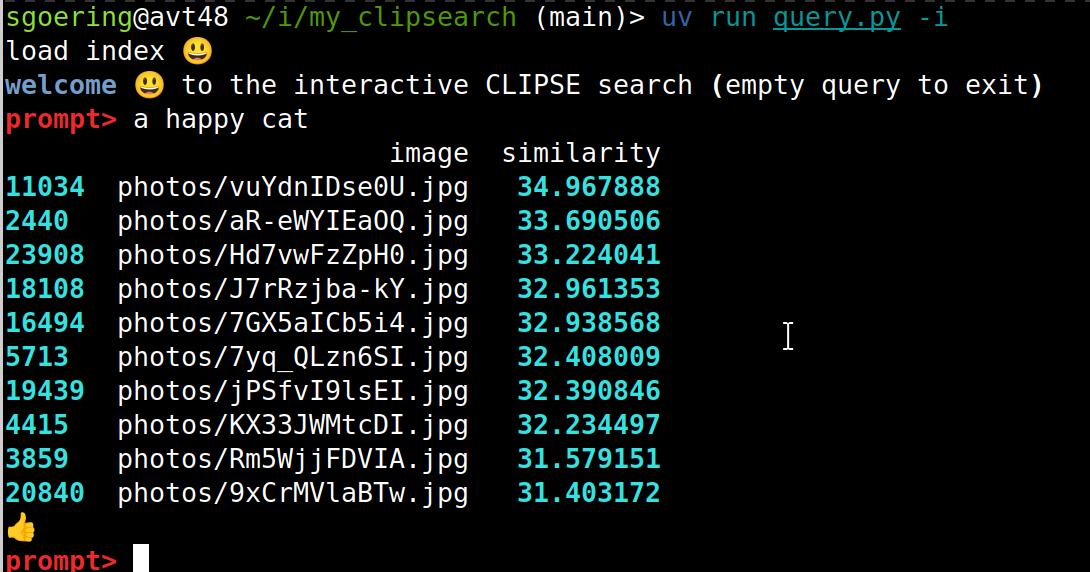
\includegraphics[width=0.5\textwidth]{CLI.jpg}
\caption{CLIPSE command line interface, example query and result.}
\label{fig:cli}
\end{figure}

The second possible interfacing way is based on a web technology \lstinline[language={bash}]{server.py}.
An example for the web interface is shown in Figure~\ref{fig:web}.

\begin{figure}
\centering
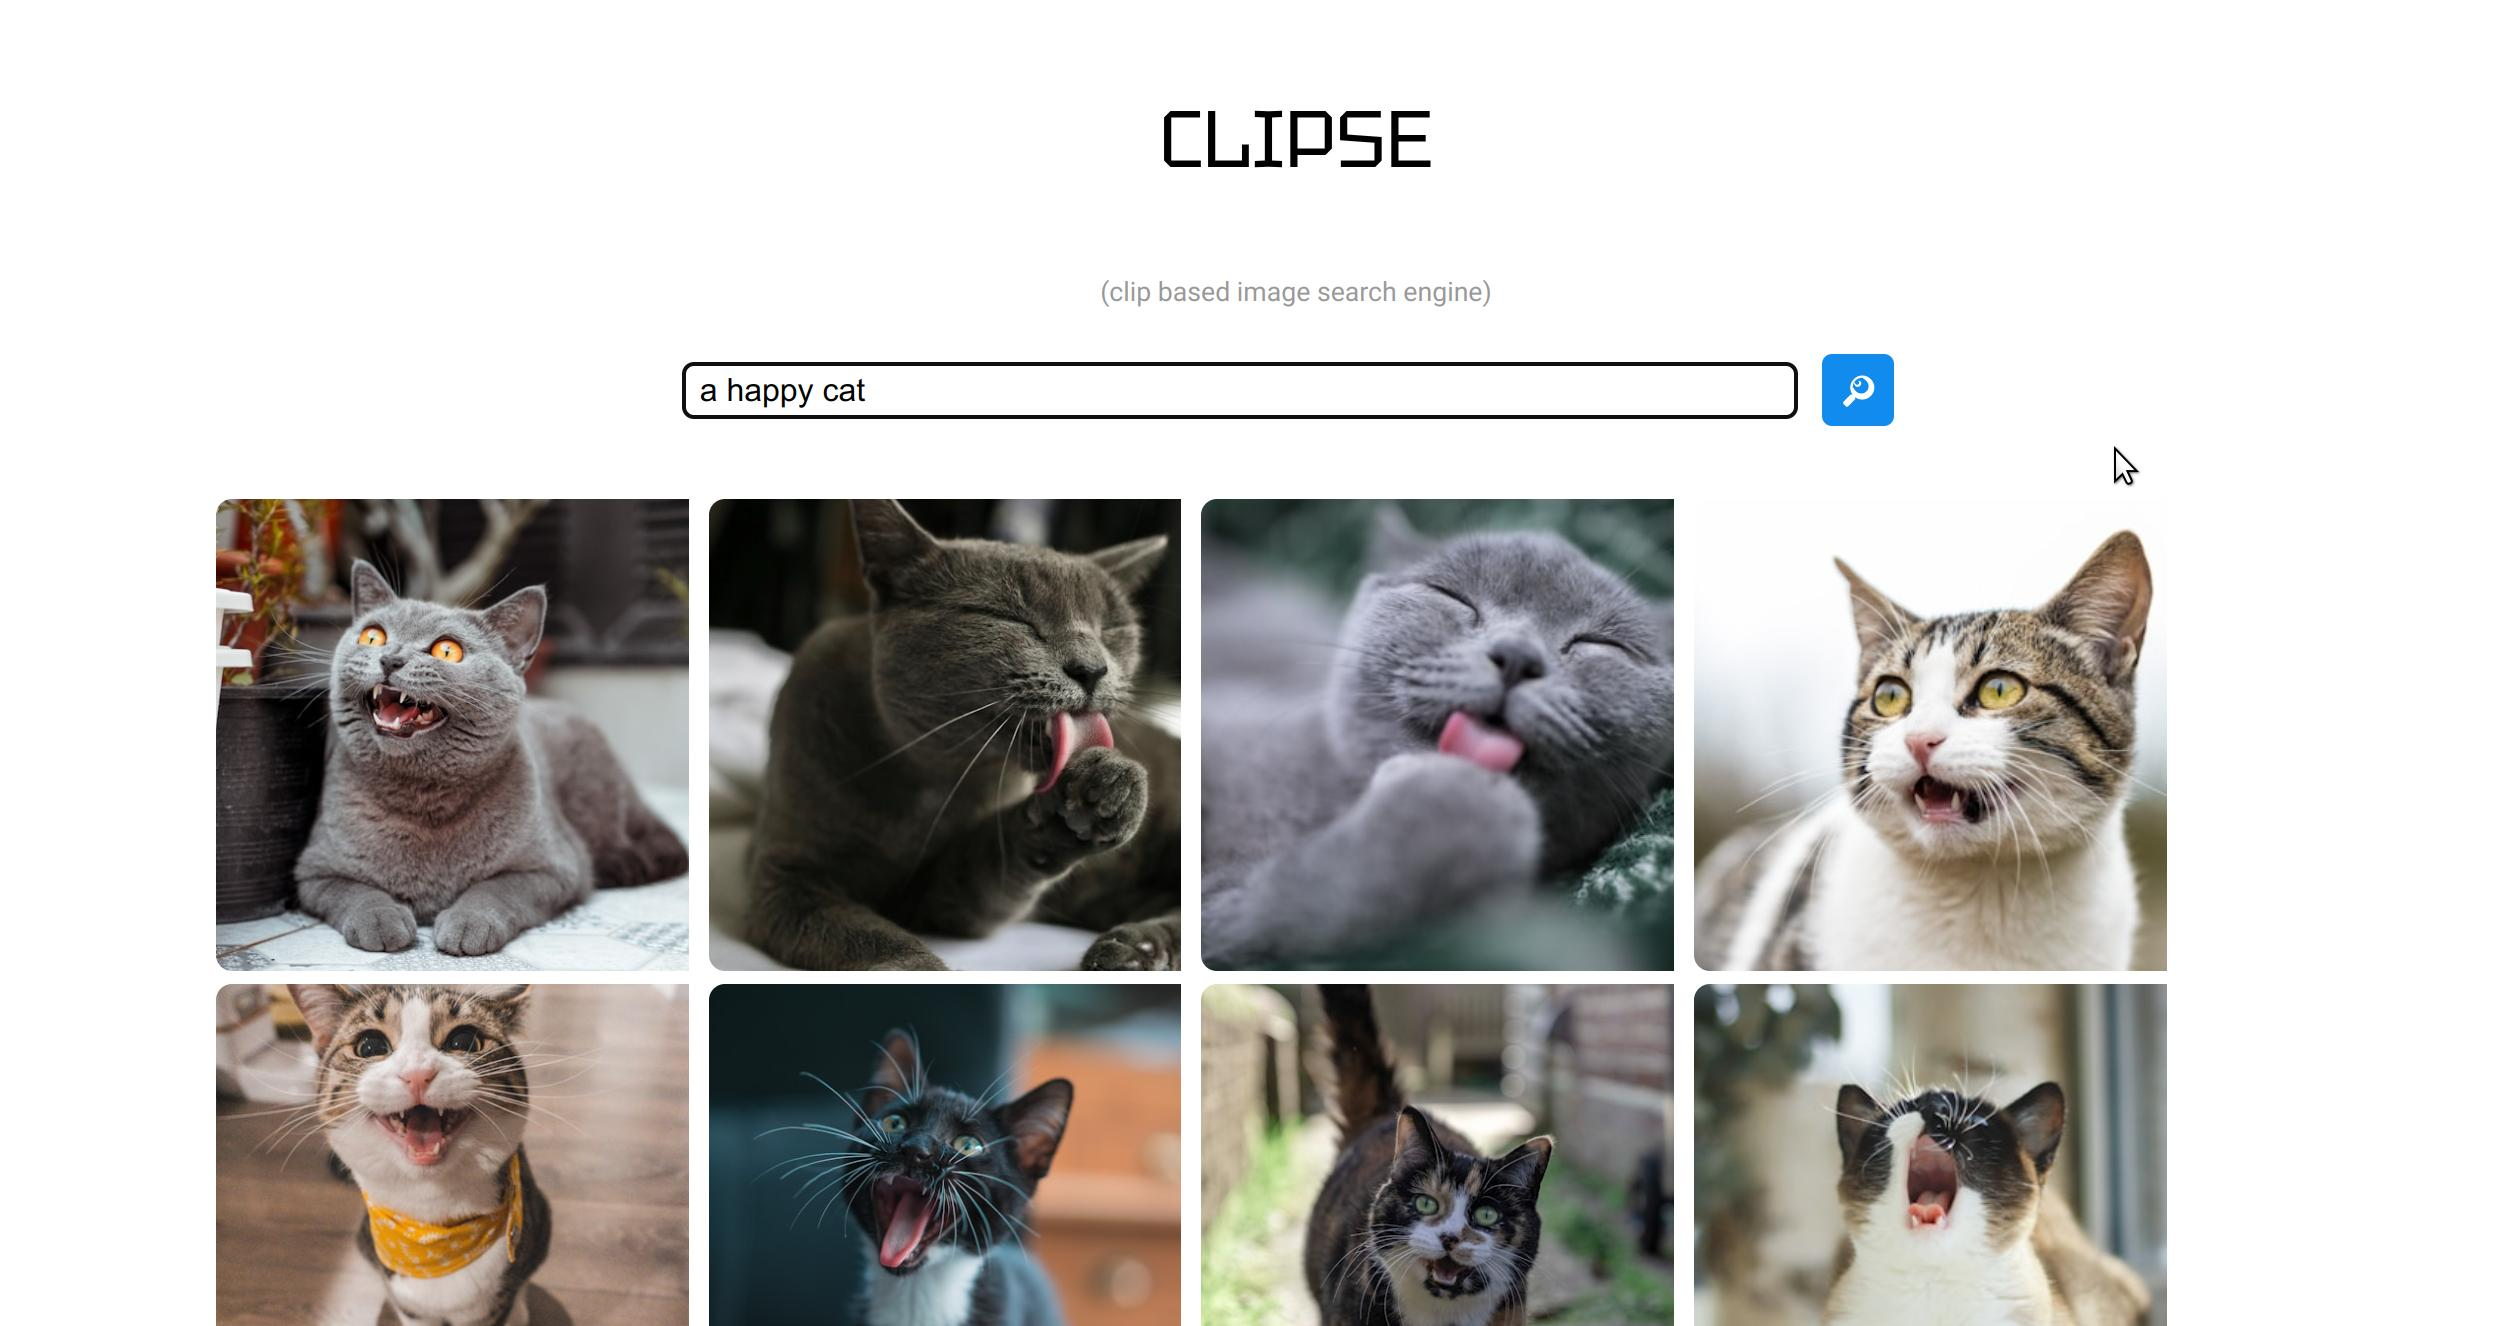
\includegraphics[width=0.85\textwidth]{WEB.jpg}
\caption{CLIPSE web interface, example query and result.}
\label{fig:web}
\end{figure}

The web-interface is based on \texttt{flask} and one simple template which uses a minimal CSS framework (\texttt{MVP}) and two JavaScript functions (one to perform the server request to gather the search results, and another one for the pagination functionality).

In both interfacing cases, the text query is transformed using OpenCLIP~\cite{ilharco_gabriel_2021_5143773,cherti2023reproducible} to the same embedding space.
Afterwards, the similarity of the text considering all images is calculated, based on the dot product.
The used dot product can be seen as an unnormalized cosine similarity measure.
Based on the similarity scores, the results are sorted and delivered as output to the corresponding interface.
Thus the performance of CLIPSE depends on the used embedding model, which can be changed in the python code.
Overall, to extend CLIPSE for very large datasets several instances could run for subsets and then a final aggregation can be performed of the results.

\section{Benchmark}


\section{Conclusion}


\bibliographystyle{alpha}
\bibliography{refs}



\end{document}
